\section{Logging Effort}

If you've done some work its a good idea to log it. In order to do this with murcs, simply navigate to that task you've been working on and press the log button (circled below).

\begin{figure}[H]
\centering
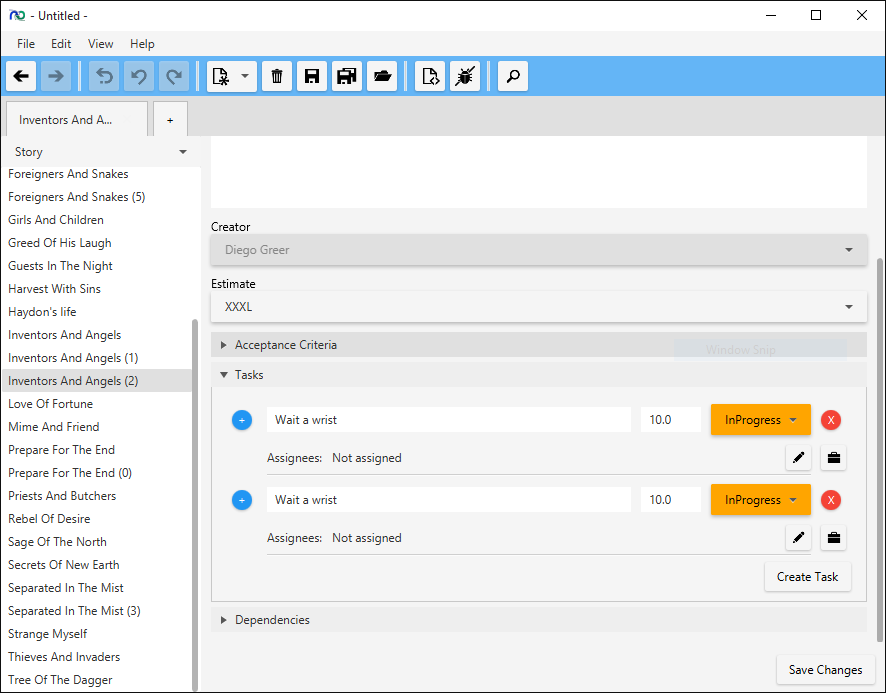
\includegraphics[width=\textwidth]{images/screenshots/logging1.PNG}
\caption{The Log Button}
\label{fig:new_project}
\end{figure}

You will be greeted with the logging effort popover. To log some effort simply enter it into the top form and press the "+" button (circled below). 

\begin{figure}[H]
\centering
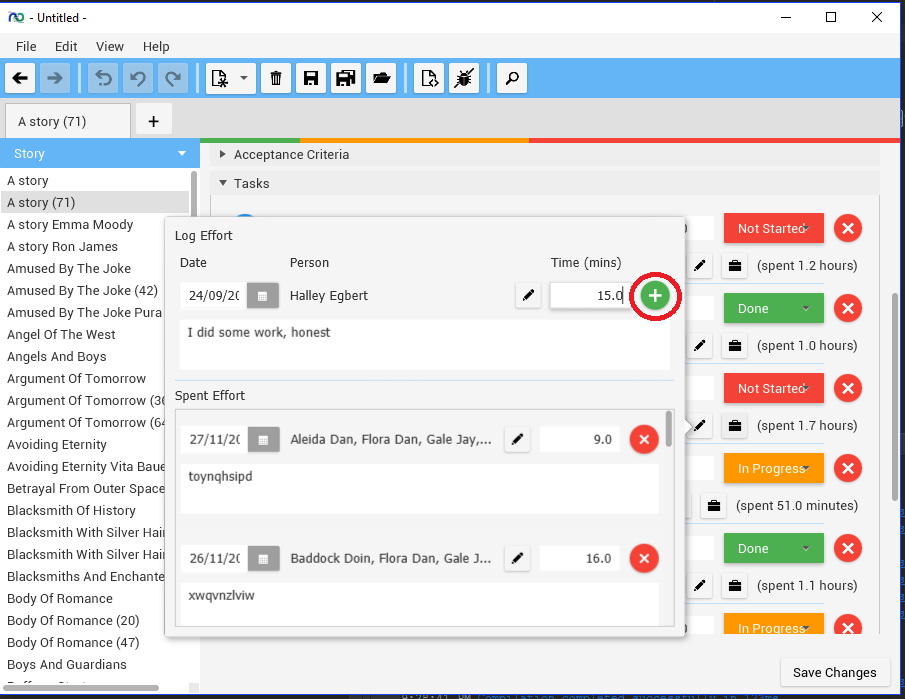
\includegraphics[width=\textwidth]{images/screenshots/logging3.png}
\caption{The Add Button}
\label{fig:new_project}
\end{figure}

Your effort will be added to the task and show up on burndowns. Effort requires a date, description, person logging effort and an amount of time (the effort). Fields with a problem will be highlighted in red.

\begin{figure}[H]
\centering
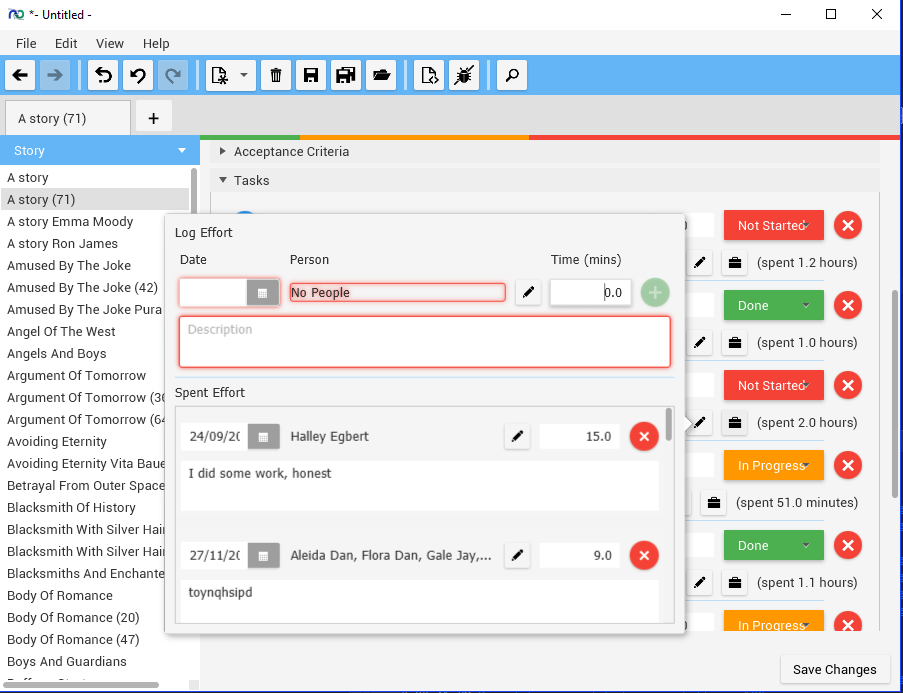
\includegraphics[width=\textwidth]{images/screenshots/logging2.png}
\caption{Form Errors}
\label{fig:new_project}
\end{figure}

All logged effort for the task shows up in the "Spent Effort" section of this form. 

\begin{figure}[H]
\centering
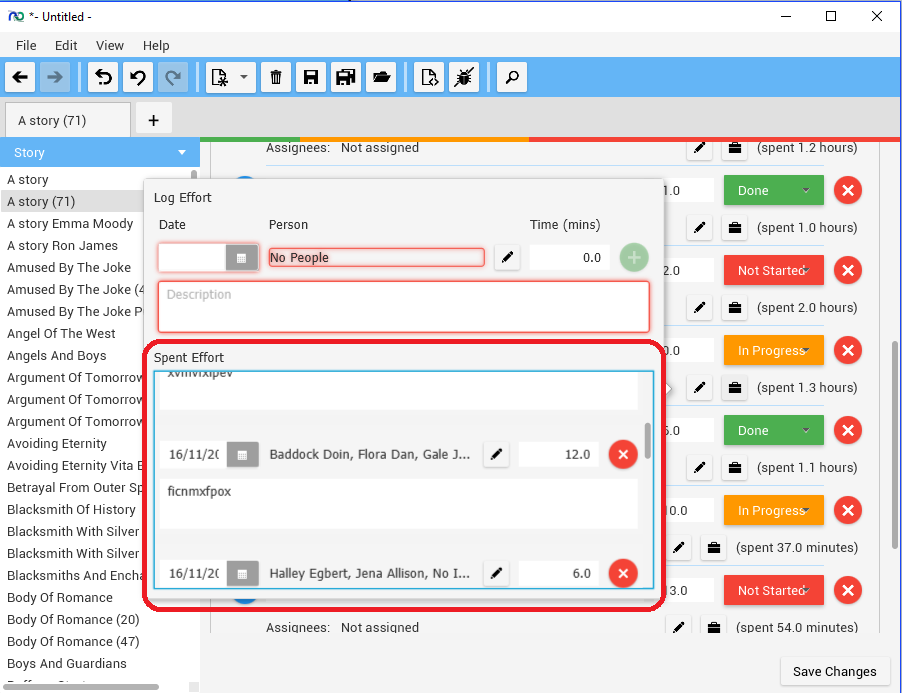
\includegraphics[width=\textwidth]{images/screenshots/logging4.png}
\caption{Spent Effort}
\label{fig:new_project}
\end{figure}

Effort can be removed using the "X" button (circled below).

\begin{figure}[H]
\centering
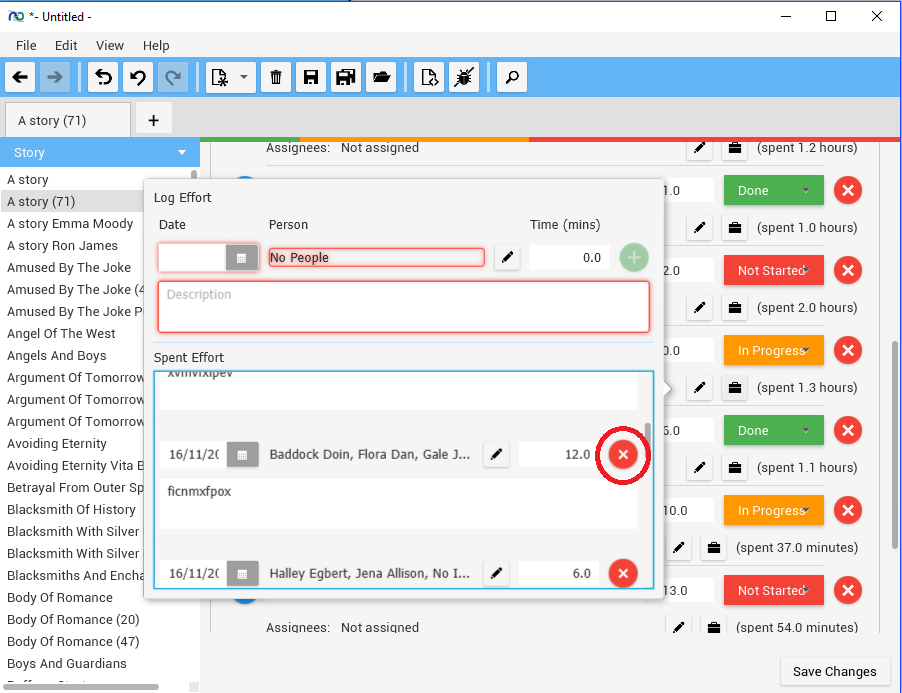
\includegraphics[width=\textwidth]{images/screenshots/logging5.png}
\caption{The Remove Button}
\label{fig:new_project}
\end{figure}